\documentclass[12pt, a4paper]{article}
\renewcommand{\figurename}{Fig.}

\usepackage[utf8]{inputenc}
\usepackage{amssymb}
\usepackage{anyfontsize}
\usepackage{lipsum}
\usepackage{graphicx}
\usepackage{subcaption}
\usepackage{geometry}
\usepackage{tikz}
\usepackage{array}
\usepackage{enumitem}

%\usepackage[showframe]{geometry}

\usetikzlibrary{automata, positioning, arrows, calc}

\geometry{top      = 2cm,
		  bottom   = 2cm,
		  left     = 2cm,
		  right    = 2cm, 
		  footskip = 1cm}


% ----- STARTING DOCUMENT ----- %

\begin{document}

\pagenumbering{arabic}

\section{Example tiles}

\noindent
In the following, $p$ will be the parameter, $x$ and $y$ will be the clocks, $a$ and $b$ two natural numbers $\in \mathbb{N}$.\\

Tile forcing the following interval: $p \in (\frac{a}{2}, \infty)$.

\begin{figure}[h!]
\begin{center}
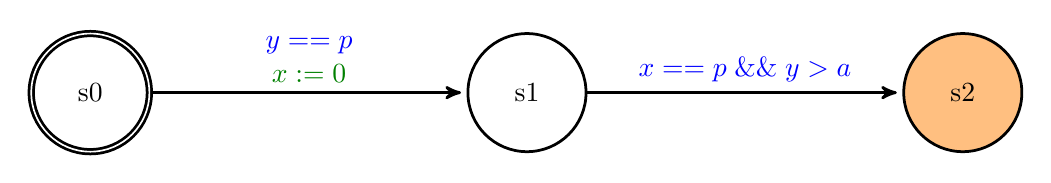
\begin{tikzpicture}
	[->,
	 >=stealth',
	 shorten >=2pt, 
	 auto,
     transform shape, 
     align=center,
     state/.style={thick, circle, draw, minimum size=1.5cm}] 
    
	\node[state, line width = 0.35mm, accepting] (s0) {s0};
	\node[state, right = 4cm of s0, line width = 0.35mm] (s1) {s1}; 
	\node[state, right = 4cm of s1, line width = 0.35mm, fill=orange!50] (s2) {s2}; 
		    
	\draw [line width=0.35mm, auto]
	(s0) edge node{\textcolor{blue}{$y == p$} \\ \textcolor{green!50!black}{$x := 0$}}(s1)
	(s1) edge node{\textcolor{blue}{$x == p \; \&\& \; y > a$}}(s2)
    ;
\end{tikzpicture}
\end{center}
\caption{Tile 2}
\label{tile 2}
\end{figure}


\bigskip

Tile forcing the following interval: $p \in (0, \frac{b}{2})$.

% In node, use accepting for initial states.
% In node, use fill=orange!50 for final states.
% In edge, use \cguard{} for guards.
% In edge, use \creset{} for assignments.

\begin{figure}[h!]
\newcommand{\cguard}{\textcolor{blue}}
\newcommand{\creset}{\textcolor{green!50!black}}

\begin{center}
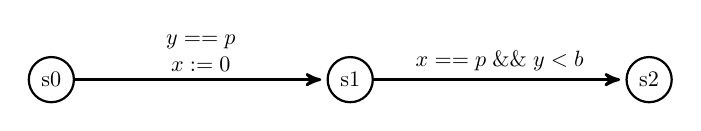
\begin{tikzpicture}[
	->,
	>=stealth',
	shorten >=2pt, 
	auto,
	scale=0.8,
    transform shape, 
    align=center,
    state/.style={thick, circle, draw}
    ] 
    
	\node[state] (s0) {s0};
	\node[state, right = 4cm of s0] (s1) {s1}; 
	\node[state, right = 4cm of s1] (s2) {s2}; 
		    
	\draw [line width=0.35mm]
	(s0) edge node{\cguard{$y == p$} \\ \creset{$x := 0$}}(s1)
	(s1) edge node{\cguard{$x == p \; \&\& \; y < b$}} (s2)
    ;
\end{tikzpicture}
\end{center}

\caption{Tile 2. Forced interval: $p \in (0, \frac{b}{2})$}
\label{tile 2}
\end{figure}



\noindent
The above tiles, namely Tile \ref{tile 1} and Tile \ref{tile 2}, can be considered as the basic building blocks for constructing every other interval, thanks to the possibility of chaining them together, hence restricting the interval in which the parameter $p$ will fall.\\

\noindent
The following one has been obtained by concatenating the aforementioned tiles.\\

Tile forcing the following interval: $p \in (\frac{a}{2}, \frac{b}{2})$.

% In node, use accepting for initial states.
% In node, use fill=orange!50 for final states.
% In edge, use \cguard{} for guards.
% In edge, use \creset{} for assignments.

\begin{figure}[h!]
\newcommand{\cguard}{\textcolor{blue}}
\newcommand{\creset}{\textcolor{green!50!black}}

\begin{center}
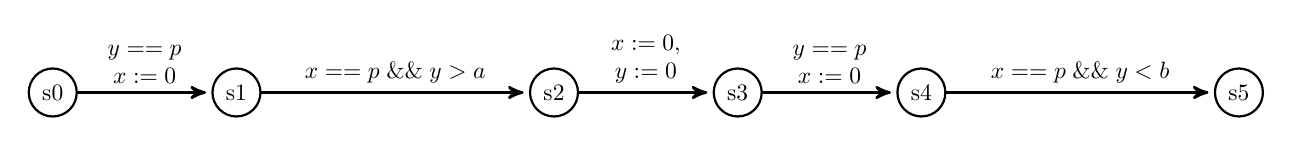
\begin{tikzpicture}[
	->,
	>=stealth',
	shorten >=2pt, 
	auto,
	scale=0.85,
    transform shape, 
    align=center,
    state/.style={thick, circle, draw}
    ] 
    
	\node[state] (s0) {s0};
	\node[state, right = 2cm of s0] (s1) {s1}; 
	\node[state, right = 4cm of s1] (s2) {s2}; 
	\node[state, right = 2cm of s2] (s3) {s3};
	\node[state, right = 2cm of s3] (s4) {s4};
	\node[state, right = 4cm of s4] (s5) {s5};   
		    
	\draw [line width=0.35mm]
	(s0) edge node{\cguard{$y == p$} \\ \creset{$x := 0$}}(s1)
	(s1) edge node{\cguard{$x == p \; \&\& \; y > a$}} (s2)
	(s2) edge node{\creset{$x := 0,$} \\ \creset{$y := 0$}} (s3)
	(s3) edge node{\cguard{$y == p$} \\ \creset{$x := 0$}}(s4)
	(s4) edge node{\cguard{$x == p \; \&\& \; y < b$}} (s5)
    ;
\end{tikzpicture}
\end{center}

\caption{Tile 3}
\label{tile 3}
\end{figure}



\noindent
Please note that Tile \ref{tile 3} can be written more concisely without using concatenation.\\

Tile forcing the following interval: $p \in (\frac{a}{2}, \frac{b}{2})$.

% In node, use accepting for initial states.
% In node, use fill=orange!50 for final states.
% In edge, use \cguard{} for guards.
% In edge, use \creset{} for assignments.

\begin{figure}[h!]
\newcommand{\cguard}{\textcolor{blue}}
\newcommand{\creset}{\textcolor{green!50!black}}

\begin{center}
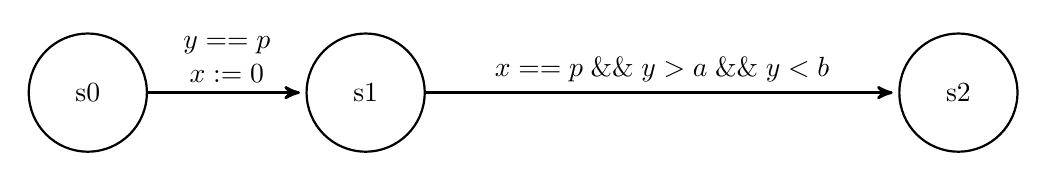
\begin{tikzpicture}[
	->,
	>=stealth',
	shorten >=2pt, 
	auto,
    transform shape, 
    align=center,
    state/.style={thick, circle, draw, minimum size=1.5cm}
    ] 
    
	\node[state] (s0) {s0};
	\node[state, right = 2cm of s0] (s1) {s1}; 
	\node[state, right = 6cm of s1] (s2) {s2};  
		    
	\draw [line width=0.35mm]
	(s0) edge node{\cguard{$y == p$} \\ \creset{$x := 0$}}(s1)
	(s1) edge node{\cguard{$x == p \; \&\& \; y > a \; \&\& \; y < b$}} (s2)
    ;
\end{tikzpicture}
\end{center}

\caption{Tile 4}
\label{tile 4}
\end{figure}



\newpage

\noindent
The following tile has 2 output states, giving rise to the ability of choosing one or the other in an OR condition.\\

Tile forcing the following interval: $p \in (0, \frac{a}{2}) \vee p \in [\frac{b}{2}, \frac{b}{2}]$.

% In node, use accepting for initial states.
% In node, use fill=orange!50 for final states.
% In edge, use \cguard{} for guards.
% In edge, use \creset{} for assignments.

\begin{figure}[h!]
\newcommand{\cguard}{\textcolor{blue}}
\newcommand{\creset}{\textcolor{green!50!black}}

\begin{center}
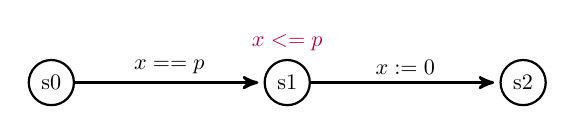
\begin{tikzpicture}[
	->,
	>=stealth',
	shorten >=2pt, 
	auto,
	scale=0.8,
    transform shape, 
    align=center,
    state/.style={thick, circle, draw}
    ] 
    
	\node[state] (s0) {s0};
	\node[state, right = 3cm of s0, label={[text=purple]$x <= p$}] (s1) {s1}; 
	\node[state, right = 3cm of s1] (s2) {s2};

	\draw [line width=0.35mm]
	(s0) edge node{\cguard{$x == p$}} (s1)
	(s1) edge node{\creset{$x := 0$}} (s2)
    ;
\end{tikzpicture}
\end{center}

\caption{Arbitrary interval Tile 5}
\label{arbitrary interval tile 5}
\end{figure}



\noindent
Please note that in such cases, unless some other previous or subsequent tile forces the parameter in a specific interval, our approach is based on trying all the parameter values starting from $n /2$ (or $n / 2 + \alpha$), so the OR tile isn't really non-deterministic in that sense. For example, testing Tile \ref{tile 5} in tChecker with values $a == 8$ and $b == 4$ the result yielded $p == 0.5$.\\

\noindent
The following tile has several inputs and outputs, being the most general type of tile we can build (one with $n$ inputs and $m$ outputs).

% In node, use accepting for initial states.
% In node, use fill=orange!50 for final states.
% In edge, use \cguard{} for guards.
% In edge, use \creset{} for assignments.

\begin{figure}[h!]
\newcommand{\cguard}{\textcolor{blue}}
\newcommand{\creset}{\textcolor{green!50!black}}

\begin{center}
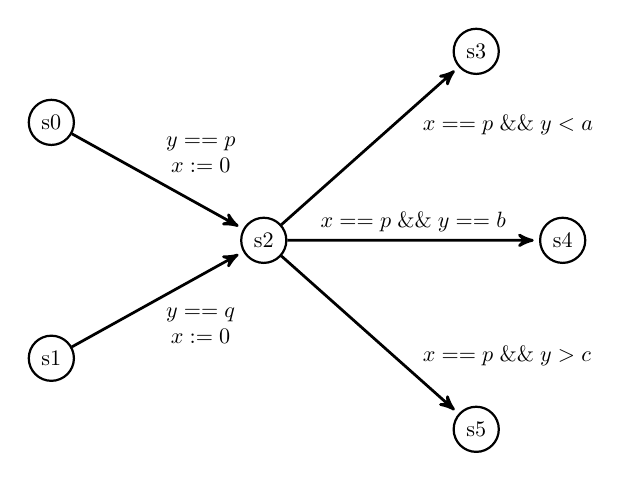
\begin{tikzpicture}[
	->,
	>=stealth',
	shorten >=2pt, 
	auto,
	scale=0.8,,
    transform shape, 
    align=center,
    state/.style={thick, circle, draw}
    ] 
    
	\node[state] (s0) {s0};
	\node[state, below = 3cm of s0] (s1) {s1}; 
	\node[state, right = 3cm of s1] (s2) at ($(s0)!0.5!(s1)$) {s2};
	\node[state, right = 3cm of s2] at ([yshift=3cm]s2) (s3) {s3}; 
	\node[state, right = 4cm of s2] (s4) {s4};
	\node[state, right = 3cm of s2] at ([yshift=-3cm]s2) (s5) {s5}; 

	\draw [line width=0.35mm]
	(s0) edge node{\cguard{$y == p$} \\ \creset{$x := 0$}}(s2)
	(s1) edge node[swap]{\cguard{$y == q$} \\ \creset{$x := 0$}} (s2)
	(s2) edge node[near end, swap]{\cguard{$x == p \; \&\& \; y < a$}} (s3)
	(s2) edge node{\cguard{$x == p \; \&\& \; y == b$}} (s4)
	(s2) edge node[near end]{\cguard{$x == p \; \&\& \; y > c$}} (s5)
    ;
\end{tikzpicture}
\end{center}

\caption{Tile 6}
\label{tile 6}
\end{figure}



\noindent
Understanding whether having multiple input states is useful or not is still under study.

\newpage

\section{Arbitrary intervals}

\noindent
Up to now, we have seen intervals such as these ones: $(0, \frac{b}{2})$ or $(\frac{a}{2}, \frac{b}{2})$, where we can notice a 2 at the denominator of the constants delimiting the interval.\\
One question that may arise is: \emph{Can such intervals be made arbitrarily small?} That is, is it possible to obtain intervals like $(\frac{a}{n}, \frac{b}{n})$, where $n \in \mathbb{N}-\{0\}$ is an arbitrarily-chosen constant?\\
Unfortunately, I don't believe this is actually possible without violating our working assumptions.\\

\noindent
In the following we recap our base assumptions on the TAs we work with:
\begin{enumerate}
\item The grammar for clock constrains does not admit algebraic operations, that is, we cannot have a clock constraint like this: $x < a + b$;
\item TAs are actually nrt-TAs, i.e. a clock cannot be reset and tested in the same transition;
\item We have only two clocks and one parameter (although the constraint on the parameter is not relevant for these considerations).
\end{enumerate}

\noindent
We have to show that it is not possible to construct a tile that is capable of forcing an arbitrarily small interval without violating any of the aforementioned assumptions.\\
For the sake of simplicity with the drawings, we will show it for the case in which $n = 3$, but a generalization of these concepts is straightforward.\\

\noindent
The first case study will try to preserve both nrt and two clocks assumptions. However, this would require illegal clock constraints syntax, as can be seen in the following figure.\\

Tile forcing the following interval: $p \in (0, \frac{a}{3})$.

\begin{figure}[h!]
\begin{center}
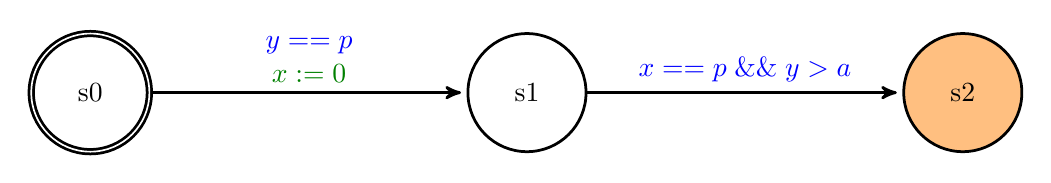
\begin{tikzpicture}
	[->,
	 >=stealth',
	 shorten >=2pt, 
	 auto,
     transform shape, 
     align=center,
     state/.style={thick, circle, draw, minimum size=1.5cm}] 
    
	\node[state, line width = 0.35mm, accepting] (s0) {s0};
	\node[state, right = 4cm of s0, line width = 0.35mm] (s1) {s1}; 
	\node[state, right = 4cm of s1, line width = 0.35mm, fill=orange!50] (s2) {s2}; 
		    
	\draw [line width=0.35mm, auto]
	(s0) edge node{\textcolor{blue}{$y == p$} \\ \textcolor{green!50!black}{$x := 0$}}(s1)
	(s1) edge node{\textcolor{blue}{$x == p \; \&\& \; y > a$}}(s2)
    ;
\end{tikzpicture}
\end{center}
\caption{Tile 2}
\label{tile 2}
\end{figure}


\noindent
Since here we let the first transition fire when y is exactly equal to p, the second transition to fire when y is exactly equal to $2p$ and the last transition to fire when x is exactly equal to $p$ and y less than $a$, since y is never reset, in the last transition it must hold that $y == 3p$. But, since we violated condition (1) above, we cannot use this construction in our analysis.\\

\noindent
Our second case study addresses the nrt nature of the TAs. It is possible to construct arbitrarily small intervals, if we get rid of the nrt property.\\

Tile forcing the following interval: $p \in (0, \frac{a}{3})$.

% In node, use accepting for initial states.
% In node, use fill=orange!50 for final states.
% In edge, use \cguard{} for guards.
% In edge, use \creset{} for assignments.

\begin{figure}[h!]
\newcommand{\cguard}{\textcolor{blue}}
\newcommand{\creset}{\textcolor{green!50!black}}

\begin{center}
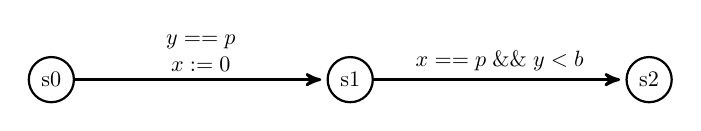
\begin{tikzpicture}[
	->,
	>=stealth',
	shorten >=2pt, 
	auto,
	scale=0.8,
    transform shape, 
    align=center,
    state/.style={thick, circle, draw}
    ] 
    
	\node[state] (s0) {s0};
	\node[state, right = 4cm of s0] (s1) {s1}; 
	\node[state, right = 4cm of s1] (s2) {s2}; 
		    
	\draw [line width=0.35mm]
	(s0) edge node{\cguard{$y == p$} \\ \creset{$x := 0$}}(s1)
	(s1) edge node{\cguard{$x == p \; \&\& \; y < b$}} (s2)
    ;
\end{tikzpicture}
\end{center}

\caption{Tile 2. Forced interval: $p \in (0, \frac{b}{2})$}
\label{tile 2}
\end{figure}



\noindent
Since in this case y is never reset, we can consider x as a sort of counter. At the end, in the last transition y will have a value corresponding to $3p$. The same considerations from the previous case also hold here. But, as mentioned at the beginning, condition (2) is violated, so we cannot use this construction in our analysis.\\

\noindent
The last case affects the number of clocks: we can get a tile forcing an arbitrarily small interval, but at the expense of adding a new clock for each natural $n \in \mathbb{N}-\{0\}$ we want to use as the denominator.\\

Tile forcing the following interval: $p \in (0, \frac{a}{3})$.

% In node, use accepting for initial states.
% In node, use fill=orange!50 for final states.
% In edge, use \cguard{} for guards.
% In edge, use \creset{} for assignments.

\begin{figure}[h!]
\newcommand{\cguard}{\textcolor{blue}}
\newcommand{\creset}{\textcolor{green!50!black}}

\begin{center}
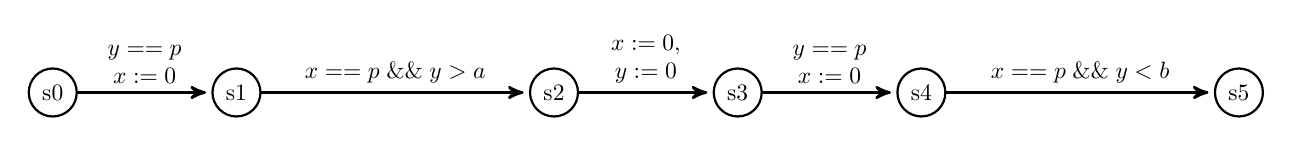
\begin{tikzpicture}[
	->,
	>=stealth',
	shorten >=2pt, 
	auto,
	scale=0.85,
    transform shape, 
    align=center,
    state/.style={thick, circle, draw}
    ] 
    
	\node[state] (s0) {s0};
	\node[state, right = 2cm of s0] (s1) {s1}; 
	\node[state, right = 4cm of s1] (s2) {s2}; 
	\node[state, right = 2cm of s2] (s3) {s3};
	\node[state, right = 2cm of s3] (s4) {s4};
	\node[state, right = 4cm of s4] (s5) {s5};   
		    
	\draw [line width=0.35mm]
	(s0) edge node{\cguard{$y == p$} \\ \creset{$x := 0$}}(s1)
	(s1) edge node{\cguard{$x == p \; \&\& \; y > a$}} (s2)
	(s2) edge node{\creset{$x := 0,$} \\ \creset{$y := 0$}} (s3)
	(s3) edge node{\cguard{$y == p$} \\ \creset{$x := 0$}}(s4)
	(s4) edge node{\cguard{$x == p \; \&\& \; y < b$}} (s5)
    ;
\end{tikzpicture}
\end{center}

\caption{Tile 3}
\label{tile 3}
\end{figure}



\noindent
Similar considerations can be done on why at the end z is equal to $3p$ (it should be trivial to notice at this stage). The tile is nrt, but having more than 2 clocks and thus violating condition (3), we cannot use this construction in our analysis.\\

\noindent
In conclusion of these considerations, it is worth noticing that, in order to construct the aforementioned illegal tiles, the number of states grows linearly with respect to the natural $n \in \mathbb{N}-\{0\}$ we want to use as the denominator: $T(n) = \Theta(n)$.\\
The same growth also happens in the case in which we opt for adding more clocks.\\
Actually, I just figured out it should be possible to obtain the same effect by using only 3 clocks: two of them are required to alternate in setting and testing the parameter (just like the first two in the example violating condition (3)), while the other clock may be used to force the interval like the z clock did in the same example.\\
Hence, attention should be put when combining them for constructing Tiled TAs, due to the growth of the states set and transitions sets (and anything related to this).

\newpage

\section{Arbitrary intervals with nrt tiles}

\noindent
It should be possible to obtain the arbitrary interval restriction while still satisfying assumptions (1), (2) and (3) above by making use of invariants and instantaneous transitions (i.e. transitions that take 0 time units to fire). However, also this construction will not be suitable for our needs, since it violates our hypothesis of time increasing strictly monotonically.\\
For the sake of completeness, we report in the following figures such construction.\\

Tile forcing the following interval: $p \in (0, \frac{a}{k})$, where $k \in \mathbb{N}-\{0\}$ (here it holds $k = 3$).

% In node, use accepting for initial states.
% In node, use fill=orange!50 for final states.
% In edge, use \cguard{} for guards.
% In edge, use \creset{} for assignments.

\begin{figure}[h!]
\newcommand{\cguard}{\textcolor{blue}}
\newcommand{\creset}{\textcolor{green!50!black}}

\begin{center}
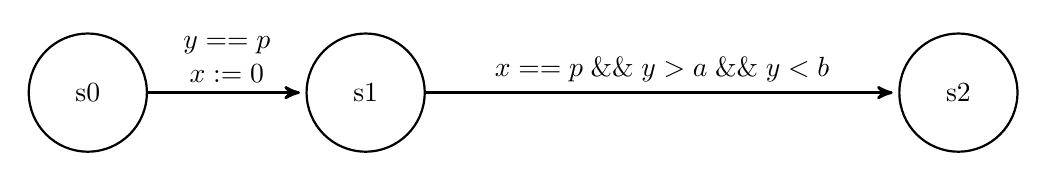
\begin{tikzpicture}[
	->,
	>=stealth',
	shorten >=2pt, 
	auto,
    transform shape, 
    align=center,
    state/.style={thick, circle, draw, minimum size=1.5cm}
    ] 
    
	\node[state] (s0) {s0};
	\node[state, right = 2cm of s0] (s1) {s1}; 
	\node[state, right = 6cm of s1] (s2) {s2};  
		    
	\draw [line width=0.35mm]
	(s0) edge node{\cguard{$y == p$} \\ \creset{$x := 0$}}(s1)
	(s1) edge node{\cguard{$x == p \; \&\& \; y > a \; \&\& \; y < b$}} (s2)
    ;
\end{tikzpicture}
\end{center}

\caption{Tile 4}
\label{tile 4}
\end{figure}



\noindent
As can be seen in the above figure, we can get an arbitrarily small interval by chaining the following sub-tile k times:

% In node, use accepting for initial states.
% In node, use fill=orange!50 for final states.
% In edge, use \cguard{} for guards.
% In edge, use \creset{} for assignments.

\begin{figure}[h!]
\newcommand{\cguard}{\textcolor{blue}}
\newcommand{\creset}{\textcolor{green!50!black}}

\begin{center}
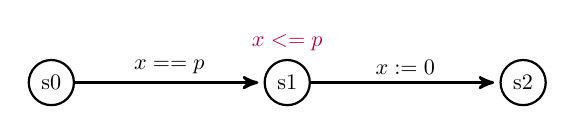
\begin{tikzpicture}[
	->,
	>=stealth',
	shorten >=2pt, 
	auto,
	scale=0.8,
    transform shape, 
    align=center,
    state/.style={thick, circle, draw}
    ] 
    
	\node[state] (s0) {s0};
	\node[state, right = 3cm of s0, label={[text=purple]$x <= p$}] (s1) {s1}; 
	\node[state, right = 3cm of s1] (s2) {s2};

	\draw [line width=0.35mm]
	(s0) edge node{\cguard{$x == p$}} (s1)
	(s1) edge node{\creset{$x := 0$}} (s2)
    ;
\end{tikzpicture}
\end{center}

\caption{Arbitrary interval Tile 5}
\label{arbitrary interval tile 5}
\end{figure}



\noindent
Notice that this ensures that at the end y (which is never reset) will have a value of $y = kp$ and thus the following holds in the last transition: $y = kp < b => p < \frac{b}{k}$, hence implying the interval mentioned above.\\
Also, here we make use of invariants in states to enforce steps every p time units, but this implies a model in which istantaneous transitions are admitted, which is not our case.\\
I have also tried reasoning on obtaining the same result with backward loops, but i fear that in this way we cannot enforce the exact interval we want.\\

\noindent
False, invariants can also be seen as guards over transitions, so the nrt property is not valid even in this case.

\newpage

\section{Tiles pre-conditions and post-conditions}

\noindent
Defining pre-conditions (and maybe also post-conditions) over the value of the clocks may be necessary in our case study.\\
As an example of pre-condition, let's take a look again at the first tile we introduced, here enriched with an extra incoming and outgoing transitions to depict the tile's pre and post-conditions.

\begin{figure}[h!]
\begin{center}
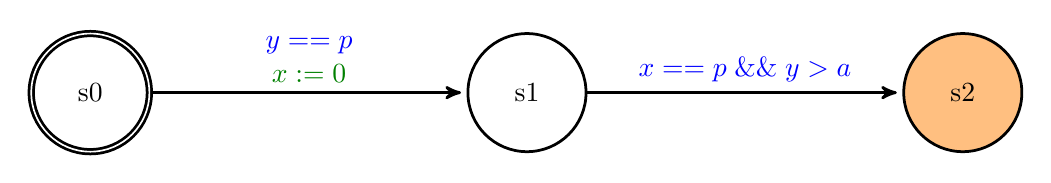
\begin{tikzpicture}
	[->,
	 >=stealth',
	 shorten >=2pt, 
	 auto,
     transform shape, 
     align=center,
     state/.style={thick, circle, draw, minimum size=1.5cm}] 
    
	\node[state, line width = 0.35mm, accepting] (s0) {s0};
	\node[state, right = 4cm of s0, line width = 0.35mm] (s1) {s1}; 
	\node[state, right = 4cm of s1, line width = 0.35mm, fill=orange!50] (s2) {s2}; 
		    
	\draw [line width=0.35mm, auto]
	(s0) edge node{\textcolor{blue}{$y == p$} \\ \textcolor{green!50!black}{$x := 0$}}(s1)
	(s1) edge node{\textcolor{blue}{$x == p \; \&\& \; y > a$}}(s2)
    ;
\end{tikzpicture}
\end{center}
\caption{Tile 2}
\label{tile 2}
\end{figure}


\noindent
A post-condition, for now, seems useless, since what's really interesting are pre-conditions; for this reason, we're going to focus on the latter.\\
Pre-conditions are interesting for this fact: if it is guaranteed that a pre-condition is met, then the behaviour of the tile is "deterministic", in the sense that it is sure (we would have to formally prove this for each tile) that, if the pre-condition requirements are met, then the parameter will always fall in the interval forced by that particular tile.\\

\noindent
Furthermore, if we can ensure that the concatenation of, let's say, Tile A with Tile B in series is such that Tile A, after executing, ensures the satisfaction of Tile B pre-conditions (and viceversa), then those two tiles may be independent from each other (we can arrange them as we want without any influence). This could lead us to formally test all single tiles without having to test the entire automaton. This should also enable us to use additional parameters, provided that we use a different parameter for each independent tile, and provided that all tiles that are used to build the TA are actually really independent.\\
This however must be formalized and maybe some small mathematical proofs must be carried out.\\

\noindent
I still am not sure what do we mean by being independent from each other: 
\begin{itemize}
\item Does this implies that we still get the same parameter interval no matter how we rearrange these tiles in the resulting TA?
\item Does this implies that the intervals do not influence each other? (but how could this be possible if for example we chain two tiles together in series?)
\end{itemize}


\noindent
Must all of this be implemented in utotparser? Maybe not, but for sure is an interesting theoretical concept I really want to include in my thesis.

\newpage

\section{Tile loops}

\noindent
Is it useful/necessary to introduce loops inside tiles?\\
First of all, if we want to perform random testing (concatenating random tiles with tiles where the parameter's interval is known), loops in such random tiles may appear but, in such a case, they would be acceptable, since randomness wouldn't be under our control.\\

\noindent
In an interval-forcing tile, however, are loops really meaningful? If the tiles' aim is only to force an interval for the parameter, maybe using a loop is redundant and not necessary.\\

\noindent
The following tile achieves the same interval as the first one introduced in this work; however, here we will use a backward loop in order to make the y clock count p time units at a time.\\

Tile forcing the following interval: $p \in (\frac{a}{2}, \infty)$.

\begin{figure}[h!]
\begin{center}
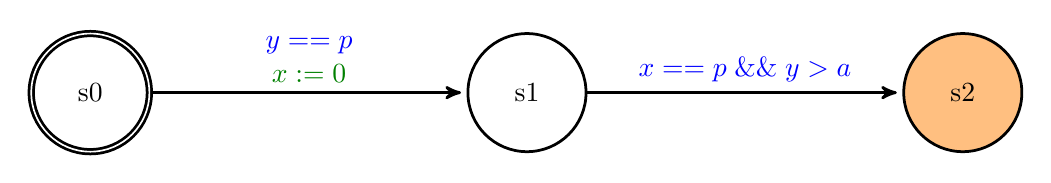
\begin{tikzpicture}
	[->,
	 >=stealth',
	 shorten >=2pt, 
	 auto,
     transform shape, 
     align=center,
     state/.style={thick, circle, draw, minimum size=1.5cm}] 
    
	\node[state, line width = 0.35mm, accepting] (s0) {s0};
	\node[state, right = 4cm of s0, line width = 0.35mm] (s1) {s1}; 
	\node[state, right = 4cm of s1, line width = 0.35mm, fill=orange!50] (s2) {s2}; 
		    
	\draw [line width=0.35mm, auto]
	(s0) edge node{\textcolor{blue}{$y == p$} \\ \textcolor{green!50!black}{$x := 0$}}(s1)
	(s1) edge node{\textcolor{blue}{$x == p \; \&\& \; y > a$}}(s2)
    ;
\end{tikzpicture}
\end{center}
\caption{Tile 2}
\label{tile 2}
\end{figure}


\noindent
As can be seen from the above tile, the use of loops makes guards on transitions shorter. This would be helpful in keeping the nrt condition (for example, the transition from s1 to s2 here only require a guard on y).\\

\noindent
However, the semantics of timed automata does not impose restrictions on how much time we can stay in a particular state, if an invariant on such a state has not been specified. Hence, here we can jump from s0 to s1 when $x == p$ but, for a suitable value of p ($p < a$), we can then wait in s1 until the condition on y is satisfied ($y > a$) and thus take the final tile transition. This suggests that, with a construction like the one above, it is not guaranteed that the parameter will stay in the pre-computed interval.\\

\noindent
We could for example take $a == 10$ and $p == 1$: in this case, when at the beginning $x == p == 1$ we would jump from s0 to s1, then wait in s1 until $y > a == 10$ and then take the transition from s1 to s2, without even entering the loop.\\
This would formally correspond to having a timed $\omega$-word with the following structure:\\
$(\pi, \tau) = (\pi_{1}, \tau_{1}) (\pi_{2}, \tau_{2}) (\pi_{n}, \tau_{n})^{\omega}$ where: $\pi_{1} = \pi_{2} = a$ and $\tau_{1} = 1, \; \tau_{2} = 11$ and $(\pi_{n}, \tau_{n})^{\omega}$ a general timed $\omega$-word.\\

\noindent
Of course, it could also happen that the loop is taken until y is of the form $y == kp$, as we proved to be the case at the beginning of this work.\\

\noindent
Speaking about loops, it is worth recalling that we may avoid loops between tiles themselves, since this could make them interact with each other, since we want to prove tile independence.





\end{document}
